%! Author = drakanoy
%! Date = 10.09.2024

% Preamble
\documentclass[12pt]{article}

% Packages
\usepackage[utf8]{inputenc}
\usepackage[T2A]{fontenc}
\usepackage[english, russian]{babel}
\usepackage[a4paper, includefoot, left=1.5cm, right=1.5cm, top=1cm, bottom=1.5cm, headsep=1cm, footskip=1cm]{geometry}
\usepackage{makecell}
\usepackage{amsmath}
\usepackage{graphicx}
\usepackage{enumitem}
\usepackage{svg}
\usepackage{multirow}
\usepackage{hyperref}
\usepackage{mathtools}
\usepackage{amssymb}
\usepackage{textcomp}
\usepackage{stmaryrd}

% Document
\begin{document}
\begin{large}
\begin{center}
\LARGE \textbf{Топология}
\par
\LARGE \textbf{Кононов Александр Михайлович}
\par
    \textbf{28.01.2025}
\end{center}
\par \textbf{Задача 1}:
\par Условие:
\par
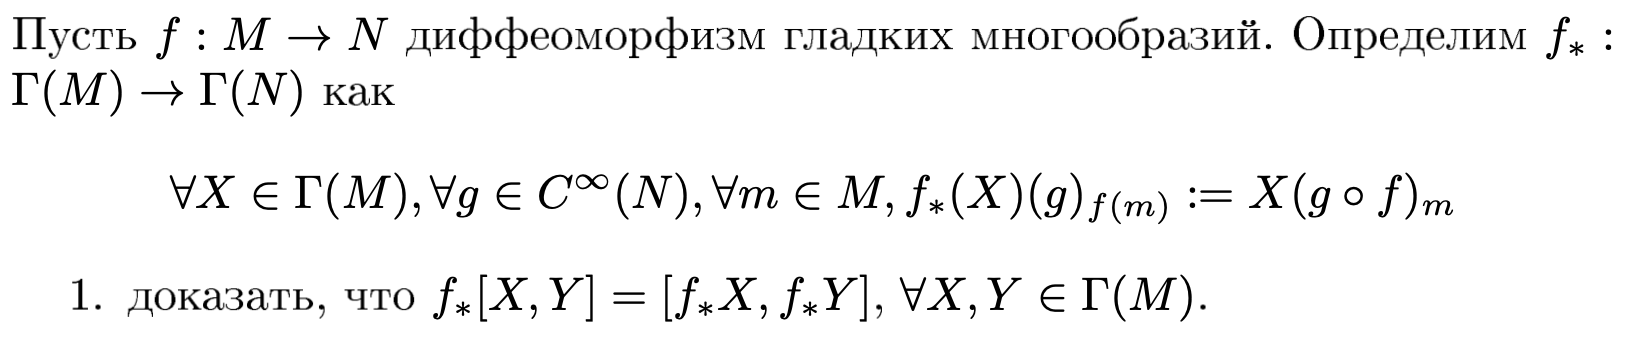
\includegraphics[width=1\textwidth]{photo_1.png}
%\begin{center}
%\underline{Рисунок 1}:
%\end{center}
\par Решение:
\par
\par
%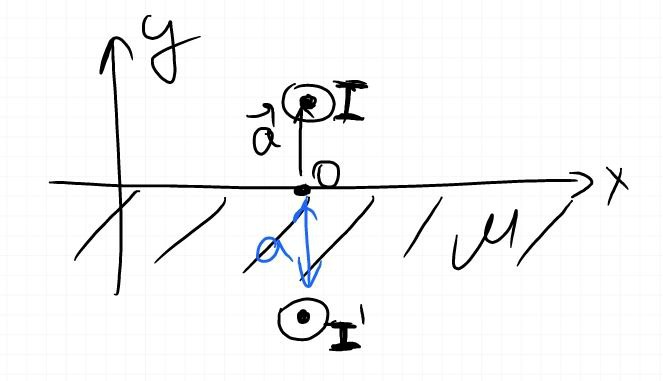
\includegraphics[width=1\textwidth]{photo_1.jpg}
%\par
%\begin{center}
%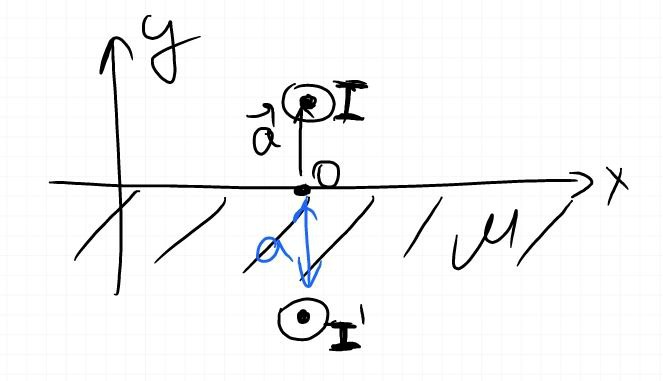
\includegraphics[width=0.4\textwidth]{photo_1.jpg}
%\end{center}
\[
    f_*(X)(g)_{f(m)} := X(g \circ f)_m
\]
\[
    (f_*(X)(g) \circ f )_{m} = X(g \circ f)_m
\]
Так как $\forall m$:
\[
    f_*(X)(g)\circ f = X(g \circ f)
\]
Теперь для $[X; Y]$:
\[
    f_*([X; Y])(g)\circ f = [X; Y](g \circ f) = ((XY) - (YX))(g \circ f) =
\]
\[
    = X(Y(g \circ f)) - Y(X(g \circ f)) = X(f_*(Y)[g] \circ f) - Y(f_*(X)[g] \circ f) =
\]
\[
    = f_*(X)[f_*(Y)[g]] \circ f - f_*(Y)[f_*(X)[g]] \circ f = (f_*(X)[f_*(Y)[g]] - f_*(Y)[f_*(X)[g]]) \circ f =
\]
\[
    = [f_*(X); f_*(Y)](g) \circ f
\]
Получили
\[
    f_*([X; Y])(g)\circ f = [f_*(X); f_*(Y)](g) \circ f \Rightarrow f_*([X; Y])(g) = [f_*(X); f_*(Y)](g)
\]
Так как для $\forall g$:
\[
    f_*([X; Y]) = [f_*(X); f_*(Y)]
\]
QED

\par \textbf{Задача 2}:
\par Условие:
\par
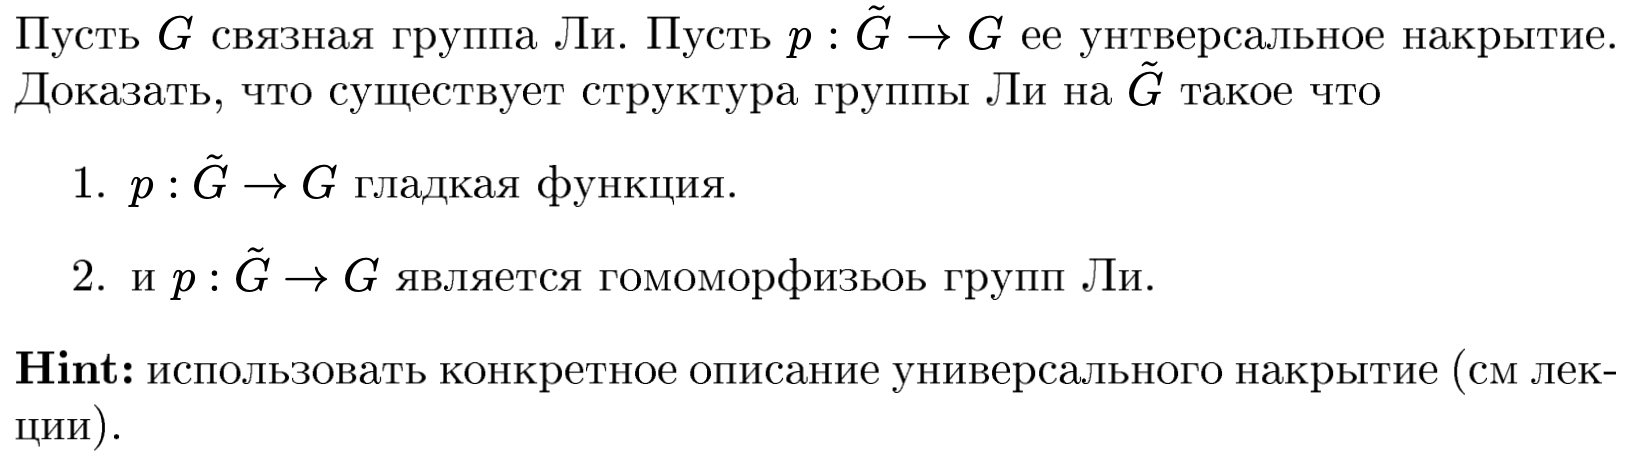
\includegraphics[width=1\textwidth]{photo_2.png}
\par Решение:
\par
\subsection*{1) Топология на $\widetilde{G}$}
Из построения универсального накрытия известно, что $\widetilde{G}$ --- топологическое пространство. Нужно лишь подтвердить три условия для гладкого многообразия:

\paragraph{1.1) Хаусдорфовость.}
Возьмём произвольные точки $x,y \in \widetilde{G}$. Пусть $p(x)=a$ и $p(y)=b$ в $G$.
\begin{itemize}
\item Если $a=b$, то берём в $G$ <<хорошую>> окрестность $U(a)$, на которой $p$ является гомеоморфизмом на соответствующих компонентах прообраза. Точки $x$ и $y$ попадают в разные компоненты, которые можно выбрать как непересекающиеся.
\item Если $a \neq b$, то в $G$ найдутся непересекающиеся <<хорошие>> окрестности $U(a)$ и $U(b)$, а в $\widetilde{G}$ --- их прообразы, которые тоже непересекаются благодаря тому, что $p$ локально является гомеоморфизмом.
\end{itemize}
Поскольку $G$ --- хаусдорфово, то и в $\widetilde{G}$ строятся непересекающиеся окрестности соответствующих точек.

\paragraph{1.2) Счётная база.}
Выберем в $G$ счётный набор <<хороших>> окрестностей $\{U_i\}$, который возможен благодаря тому, что $G$ имеет счётную базу. Тогда прообраз каждой $U_i$ под $p$ раскладывается в дизъюнктное объединение $U_{i,j}$:
\[
p^{-1}(U_i) = \bigsqcup_j U_{i,j}.
\]
Все такие $U_{i,j}$ вместе образуют счётную базу на $\widetilde{G}$.

\paragraph{1.3) Атлас на $\widetilde{G}$.}
Пусть $x \in \widetilde{G}$ и $p(x)=a$. Так как $a$ имеет <<хорошую>> окрестность $U(a)$ в $G$ и $p$ при этом локальный гомеоморфизм, рассмотрим соответствующий кусок $V_x \subset \widetilde{G}$, который отображается гомеоморфно на $U(a)$.

В $G$ уже есть гладкая структура с атласом $\{\varphi_i\}$. Тогда на каждом $V_x$ зададим карты
\[
\widetilde{\varphi}_i = \varphi_i \circ p \bigl|_{V_x}.
\]
Композиция гомеоморфизма и гладкой карты даёт гладкую карту. Собирая такие карты по всем <<хорошим>> окрестностям и их прообразам, получаем полный атлас на $\widetilde{G}$. Согласованность новых карт получается из согласованности исходных $\varphi_i$.

\subsection*{2) Гладкость $p \colon \widetilde{G} \to G$}
Чтобы проверить гладкость $p$, достаточно проверить гладкость его локальных версий в координатных картах. Но локально $p$ --- композиция уже гладких (или гомеоморфных) отображений, следовательно, гладкое.

\subsection*{3) Групповая операция и обращение}
На $\widetilde{G}$ определяется умножение
\[
\widetilde{\mu}\bigl([\alpha(t)], [\beta(t)]\bigr) = \bigl[\alpha(t)\,\beta(t)\bigr],
\]
где $[\alpha(t)]$ и $[\beta(t)]$ --- классы петель в $G$. Корректность: гомотопные петли при умножении дают гомотопные результаты. Нейтральным элементом выступает класс $\bigl[e_c(t)\bigr]$, где $e_c(t)$ --- постоянный путь в нейтральном элементе $G$. Обращение петли $[\alpha(t)]$ задаётся путём
\[
[\alpha(t)]^{-1} = \bigl[\alpha(t)^{-1}\bigr].
\]

\subsection*{4) Гладкость $\widetilde{\mu}$ и $\widetilde{\mathrm{inv}}$}
\paragraph{4.1) Гладкость $\widetilde{\mu}$.}
Умножение на $G$ есть гладкое отображение $\mu \colon G \times G \to G$. На $\widetilde{G} \times \widetilde{G}$ по определению
\[
\mu \;=\; p \;\circ\; \widetilde{\mu}\;\circ\;(p^{-1} \times p^{-1}),
\]
и поскольку локально все карты согласованы с картами в $G \times G$, операция $\widetilde{\mu}$ получается гладкой.

\paragraph{4.2) Гладкость $\widetilde{\mathrm{inv}}$.}
Аналогично, $\mathrm{inv} \colon G \to G$ гладко. Тогда
\[
\mathrm{inv} \;=\; p \;\circ\; \widetilde{\mathrm{inv}} \;\circ\; p^{-1}.
\]
В локальных координатах эта композиция диффеоморфизмов также гладкая, значит, и $\widetilde{\mathrm{inv}}$ гладко.

Таким образом, на $\widetilde{G}$ формируется структура группы Ли.

\subsection*{5) Гомоморфизм групп Ли}
Наконец, покажем, что $p \colon \widetilde{G} \to G$ --- гомоморфизм групп Ли. Мы уже доказали его гладкость. Для свойств гомоморфизма надо лишь проверить согласованность умножений:
\[
p\Bigl([\alpha(t)] \cdot [\beta(t)]\Bigr) \;=\; p\Bigl([\alpha(t)\,\beta(t)]\Bigr)
\;=\; \alpha(1)\,\beta(1)
\;=\; p([\alpha(t)])\;\cdot\;p([\beta(t)]).
\]
Значит, $p$ действительно переводит произведение в произведение, то есть является гомоморфизмом групп Ли. QED

\par \textbf{Задача 3}:
\par Условие:
\par
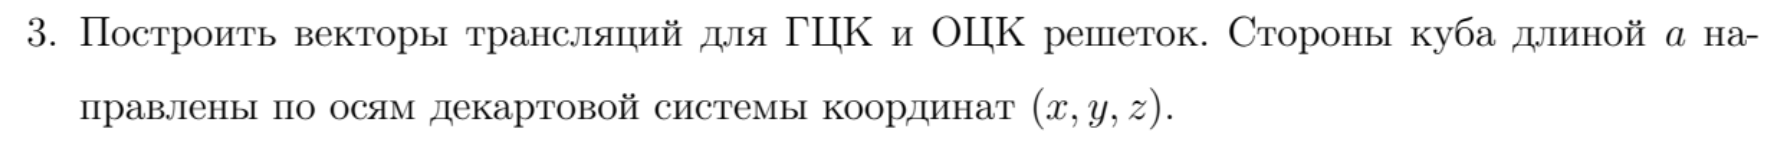
\includegraphics[width=1\textwidth]{photo_3.png}
\par Решение:
\par 1) Покажем компактность:
\[
    (X \times Y, \tau)
\]
\[
    (X, \Omega) - \text{компакт}
\]
\[
    (Y, \varSigma) - \text{компакт}
\]
\[
    \forall \nu = \{ U_i \in \Omega \mid i \in I \, ; \, \, \bigcup\limits_{i \in I} U_i = X \} \, \, \, \exists U_{i_1}; ...; U_{i_n} \in \nu \, \, \, \bigcap\limits_{i = 1}^n U_i = X - \text{конеч подпокрытие}
\]
\[
    \forall \eta = \{ V_j \in \varSigma \mid j \in J \, ; \, \, \bigcup\limits_{j \in J} V_j = Y \} \, \, \, \exists V_{j_1}; ...; V_{j_m} \in \nu \, \, \, \bigcap\limits_{j = 1}^m V_j = Y - \text{конеч подпокрытие}
\]
\[
    \mu = \{ W_k \in \tau \mid k \in K \, ; \, \, \bigcup\limits_{k \in K} W_k = X \times Y \} - \text{покрытие}
\]
\[
    \forall W_k = U_k \times V_k - \text{декартова топология}
\]
\[
    U_k; \,\,\, k \in K - \text{откр покрытие} X \Rightarrow \exists U_{k_1}; ...; U_{k_n} - \text{конеч подпокрытие} X
\]
\[
    V_k; \,\,\, k \in K - \text{откр покрытие} Y \Rightarrow \exists V_{k_1}; ...; V_{k_m} - \text{конеч подпокрытие} Y
\]
\[
    \Rightarrow \tau \supset \tau_{n;m} = \{ W_{k_{i; j}} = U_{k_i} \times V_{k_j} \mid i \in \{1; ...; n\}; j \in \{1; ...; m\} \} - \text{конеч подпокрытие} X \times Y
\]
QED
\par 2) Покажем связность:
\par От противного. Пусть $\tau$ - несвязна. Тогда:
\[
    \exists a = (x_1; y_1); b = (x_2; y_2) : \forall A \in \tau \, \, \, a; b \notin A
\]
Связность $X$ и $Y$:
\[
    \forall x_1; x_2 \in X \, \, \,  \exists A_x \in \Omega : \, \, \, x_1; x_2 \in A_x
\]
\[
    \forall y_1; y_2 \in Y \, \, \,  \exists A_y \in \varSigma : \, \, \, y_1; y_2 \in A_y
\]
\[
    \Rightarrow A' = \{ (x;y) \in X \times Y \mid x = x_1\} \, \, \, A'' = \{ (x;y) \in X \times Y \mid y = y_2\} - \text{связаны}
\]
\[
    A' \bigcap A'' = \{(x_1; y_2)\} \neq \varnothing \Rightarrow_{\text{крит связ}} X \times Y - \text{связное} %a\, \, \, QED
\]
\par QED
\par \textbf{Задача 4}:
\par Условие:
\par
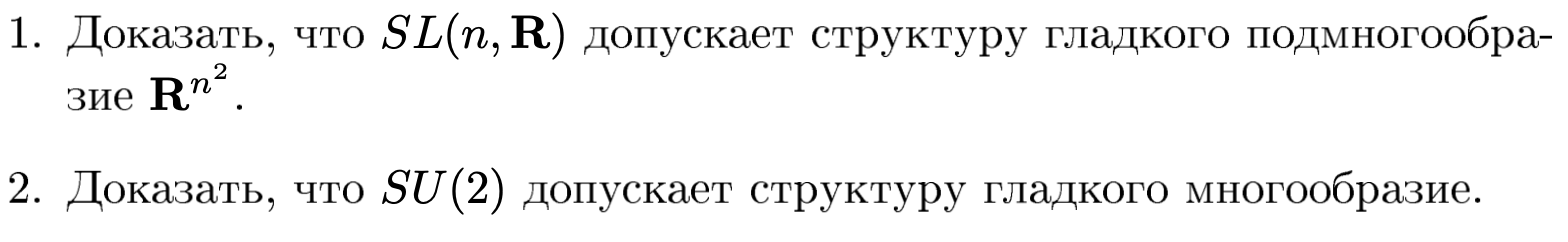
\includegraphics[width=1\textwidth]{photo_4.png}
\par Решение:
\par 1) $SL_n(\mathbb{R})$:
\[
    det : \mathbb{R}^{n^2} \longrightarrow \mathbb{R}
\]
\[
    M \longmapsto det(M) = \sum\limits_{\sigma \in S_n} sgn (\sigma) \cdot \prod\limits_{i = 1}^n a_{i \sigma(i)}
\]
\[
    SL_n(\mathbb{R}) = det^{-1}(1)
\]
Докажем, что $1 \in \mathbb{R}$ - регулярное значение $det$.
\[
    D_{M}det = \nabla det(M) = \left( \frac{\partial det}{\partial x_{11}}; \dotso; \frac{\partial det}{\partial x_{nn}}  \right)(M)
\]
\[
    \forall M \in SL_n(\mathbb{R}) \, \, \,  \nabla det(M) \neq 0 \Rightarrow Rank \nabla det = 1
\]
Значит любая точка $SL_n(\mathbb{R})$ регулярная. По теореме о регулярном значении функции между многообразиями $SL_n(\mathbb{R})$ - гладкое подмногообразие $\mathbb{R}^{n^2}$. QED
\par 2) $SU(2)$:
\begin{equation*}
    SU(2)
    = \left\{
    \begin{pmatrix}
        a & -\overline{b}\\
        b & \overline{a}
    \end{pmatrix}
    \Bigg| a; b \in \mathbb{C}; \,\,\, |a|^2 + |b|^2 = 1
    \right\}
\end{equation*}
\[
    SU(2) \subseteq \mathbb{C}^4 \cong \mathbb{R}^8
\]
\[
    S^3 = \{ (x; y; z; t) \in \mathbb{R}^4 \mid x^2 + y^2 + z^2 + t^2 = 1 \}
\]
\[
    f : S^3 \longrightarrow SU(2) \subseteq \mathbb{R}^8
\]
\begin{equation*}
    (x; y; z; t) \longmapsto
    \begin{pmatrix}
        x + iy & -z+it\\
        z+it & x-iy
    \end{pmatrix} - \text{непр, биекция}
\end{equation*}
\[
    \Rightarrow SU(2) \cong S^3
\]
\[
    g : S^3 \longrightarrow \mathbb{R}
\]
\[
    (x; y; z; t) \longmapsto x^2 + y^2 + z^2 + t^2
\]
\[
    SU(2) = g^{-1}(1)
\]
Докажем, что $1 \in \mathbb{R}$ - регулярное значение $g$.
\[
    \nabla g = (2x; 2y; 2z; 2t) \neq 0 \, \, \, \, \forall (x; y; z; t) \in SU(2)
\]
\par Теорема регулярном значении функции между многообразиями
\par $\Rightarrow$ QED

\par \textbf{Задача 5}:
\par Условие:
\par
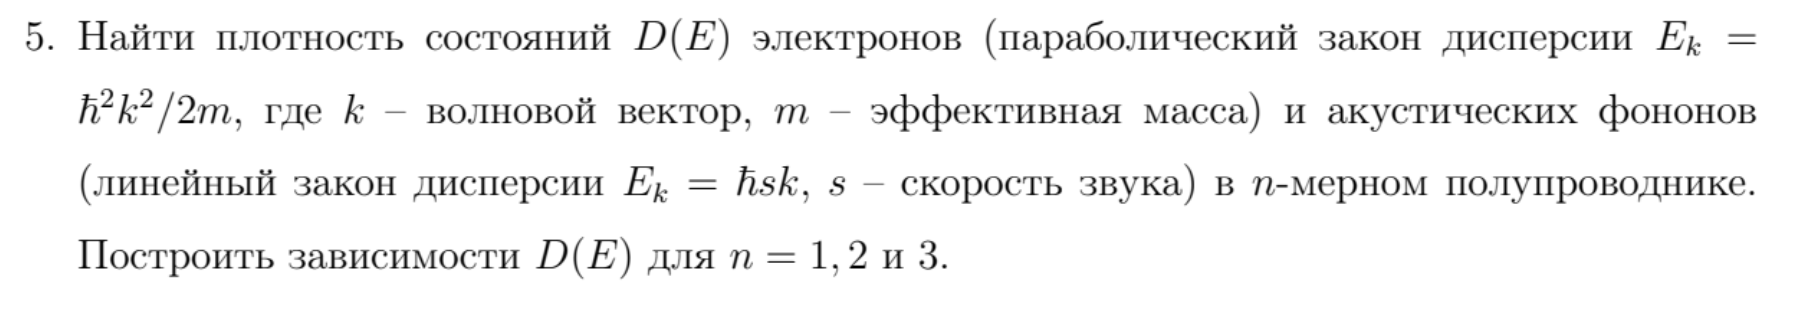
\includegraphics[width=1\textwidth]{photo_5.png}
\par Решение:
\par От противного. Пусть $\mathbb{R}^2 \overset{f}{\simeq} \mathbb{R}^5$ - гомеоморфны.
\par Тогда
\[
    \mathbb{R}^2 - \{0\} \overset{f}{\simeq} \mathbb{R}^5 - \{f(0)\} \Leftrightarrow \mathbb{R}^2 - \{0\} \overset{f}{\simeq} \mathbb{R}^5 - \{0\}
\]
Знаем
\[
    \mathbb{R}^2 - \{0\} \simeq S^1
\]
\[
    \mathbb{R}^5 - \{0\} \overset{g}{\simeq} S^4
\]
\[
    g: \vec{x} \longmapsto \frac{\vec{x}}{x}
\]
\[
    S^4 \hookrightarrow \mathbb{R}^5
\]
\[
    \Rightarrow \mathbb{Z} = \pi_1\left( S^1; \vec{x} \right) = \pi_1\left( \mathbb{R}^2 - \{0\}; \vec{x} \right) = \pi_1\left( \mathbb{R}^5 - \{0\}; f(\vec{x}) \right) = \pi_1\left( S^4; \frac{f(\vec{x})}{|f(\vec{x})|} \right) = 0
\]
\par Противоречие. QED

\par \textbf{Задача 6}:
\par Условие:
\par
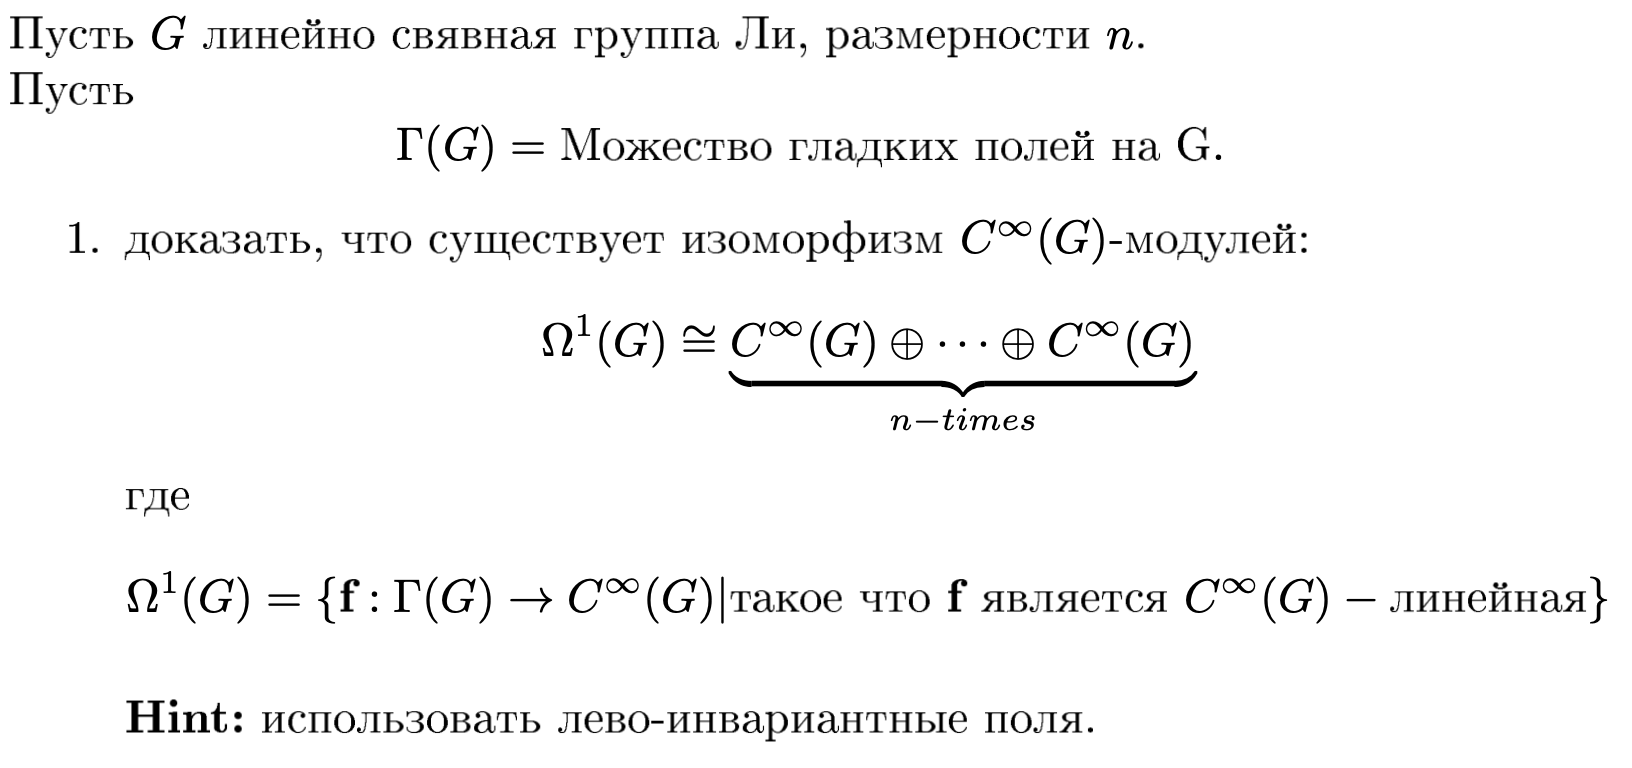
\includegraphics[width=1\textwidth]{photo_6.png}
\par Решение:
\par Обозначим за $\mathfrak{g} = T_e G$ алгебру Ли в единице $e\in G$ и выберем базис
$\{X_1;\dots;X_n\}\subset \mathfrak{g}$.
Для каждого $i$ определим лево-инвариантное поле $\widetilde{X}_i$ на $G$ путём переноса $X_i$ с помощью левых сдвигов.
Тогда $\{\widetilde{X}_1;\dots;\widetilde{X}_n\}$ образуют базис в $\Gamma(G)$.
\par Любое векторное поле $Y\in \Gamma(G)$ можно разложить в этом базисе:
\[
    Y[f](g) \;=\;\sum_{j=1}^n a_j(g)\,\widetilde{X}_j[f](g) \quad \text{где } a_j \in C^\infty(G) \; \forall f \in C^\infty(G) \; \forall g \in G
\]

Рассмотрим 1-форму $\omega \in \Omega^1(G)$. По опруделению:
\[
    \omega \left( h Y + k Z \right) = h \omega \left( Y \right) + k \omega \left( Z \right) \; \forall h; k \in C^\infty(G) \; Y; Z \in \Gamma(G)
\]
Определим \(\omega\) на базисных полях \(X_j\) и получим \(n\) гладких функций:
\[
\omega(X_j)\;\in\;C^\infty(G),\quad j=1,\dots,n.
\]
Зададим отображение
\[
\Phi \colon \Omega^1(G) \;\longrightarrow\;\bigl(C^\infty(G)\bigr)^n,
\quad
\omega \;\mapsto\;\bigl(\omega(X_1),\dots,\omega(X_n)\bigr).
\]
Проверим биективнось:
\par 1) Инъективность:
\[
    \omega(\widetilde{X}_j)=0 \Rightarrow \omega \left(\sum_{j=1}^n a_j(g) \,\widetilde{X}_j[f](g) \right) = 0 \Rightarrow \omega = 0
\]
\par 2) Сюрьективность:
\[
    \omega(\widetilde{X}_j) \;=\; f_j \Rightarrow \; \forall Y = \sum_j a_j \widetilde{X}_j \, \, \, \, \omega(Y) = \sum_j a_j f_j \in \Omega^1(G)
\]
Получили
\[
    \Omega^1(G) \cong \bigoplus_{i=1}^n C^\infty(G)
\]
По сути доказали:
\[
    \Omega^1(G) = \Gamma(G)^*
\]
QED

\par \textbf{Задача 7}:
\par Условие:
\par
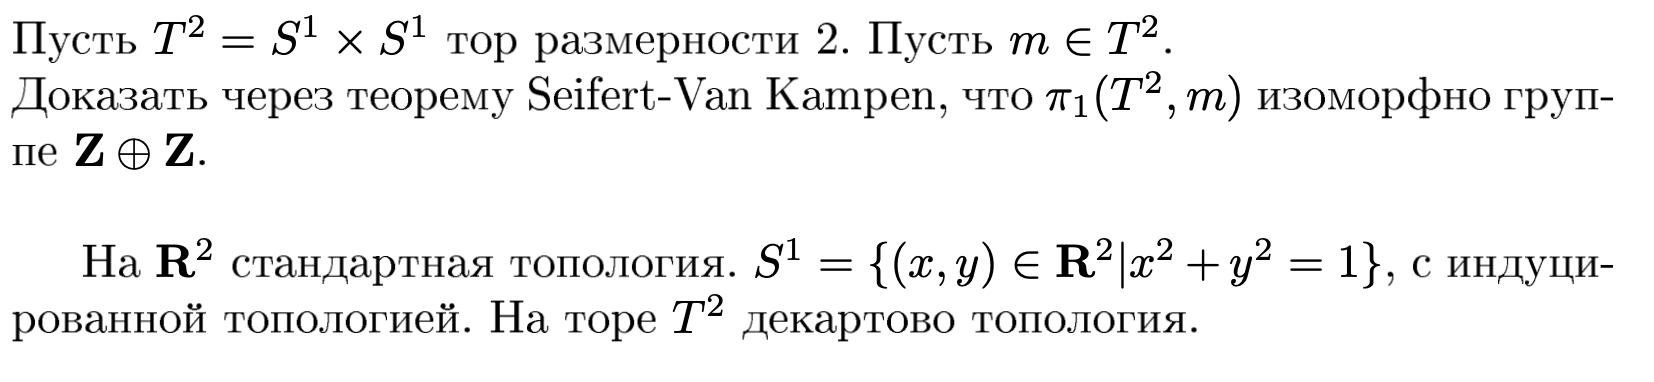
\includegraphics[width=1\textwidth]{photo_7.png}
\par Решение:
\[
    \mathbb{T}^2 \cong [0; 1] \times [0; 1]/ \sim  \text{с фактор топологией}
\]
\[
    (0; s) \sim (1; s) \; (t; 0) \sim (t; 1) \, \, \, \forall t ; s \in [0; 1]
\]
\[
    U_1 = \mathbb{T}^2 - \{M\} - \text{откр, лин связ}
\]
\[
    U_2 = B_{\varepsilon}(M) - \text{откр, лин связ}
\]
\[
    U_1 \bigcap U_2 = U_2 - \{M\} - \text{откр, лин связ}
\]
По Теореме Ван-Кампана:
\par
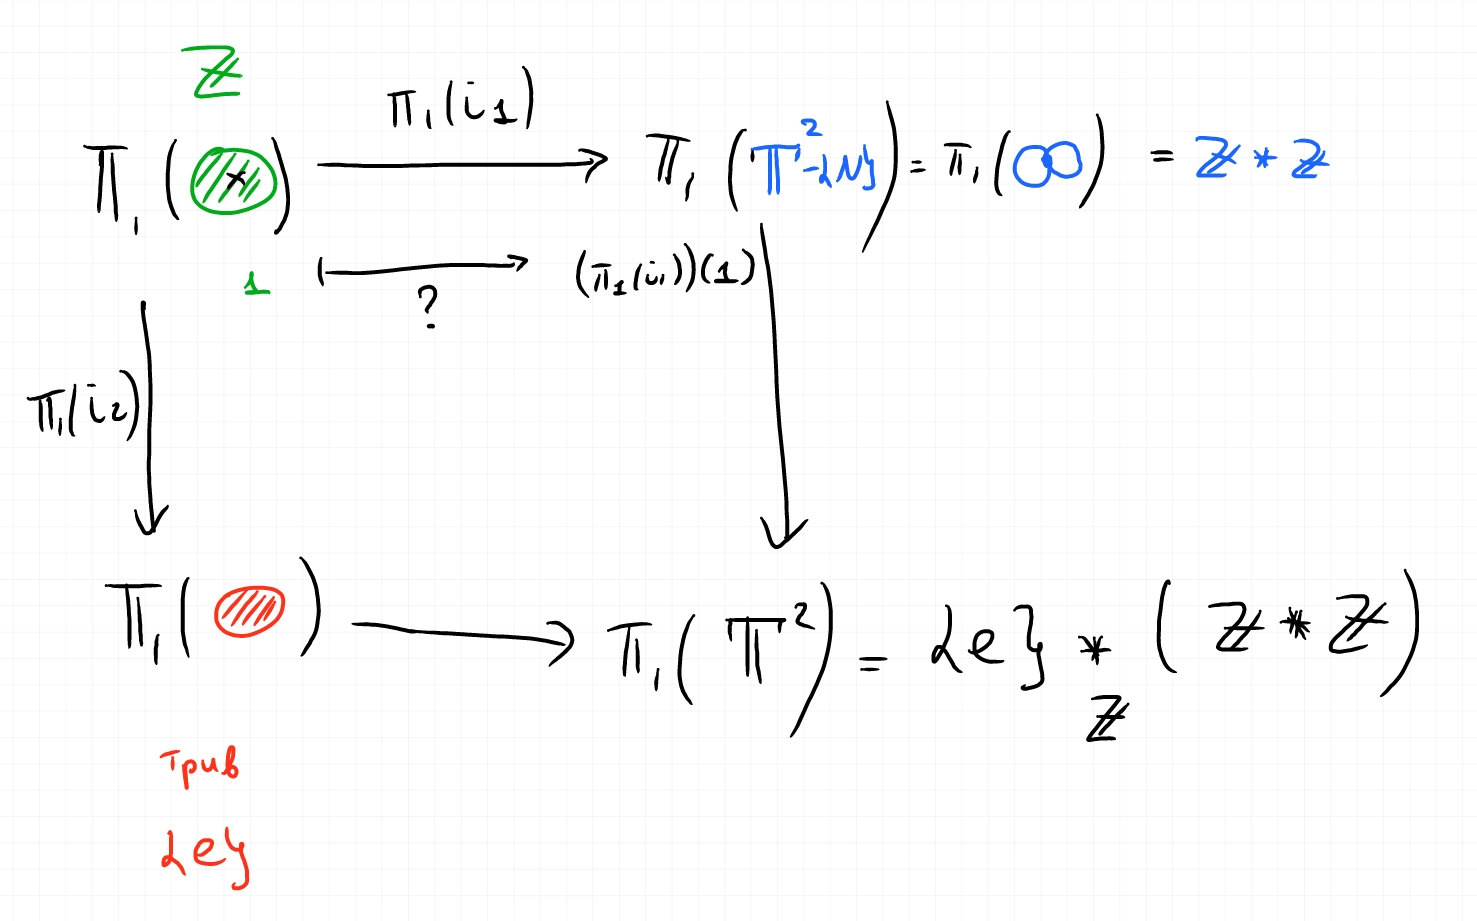
\includegraphics[width=1\textwidth]{photo_71.jpg}
\par
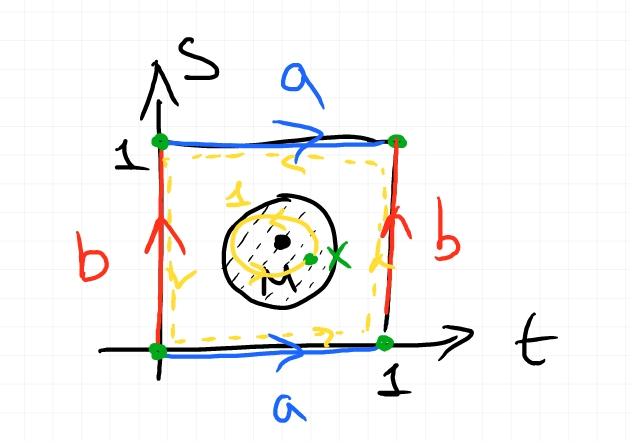
\includegraphics[width=1\textwidth]{photo_72.jpg}
\par Чтобы получить генератор $\mathbb{Z}$ - обойдем тор по петле
\[
    \Rightarrow 1 \overset{\pi_1(i_1)}{\longmapsto} aba^{-1}b^{-1}
\]
\[
    \Rightarrow \pi_1(\mathbb{T}^2) = \{e\} \underset{\mathbb{Z}}{*} (\mathbb{Z} * \mathbb{Z}) = \left< a; b \mid aba^{-1}b^{-1} \right> = \mathbb{Z} \oplus \mathbb{Z}
\]
\par QED

\par \textbf{Задача 8}:
\par Условие:
\par
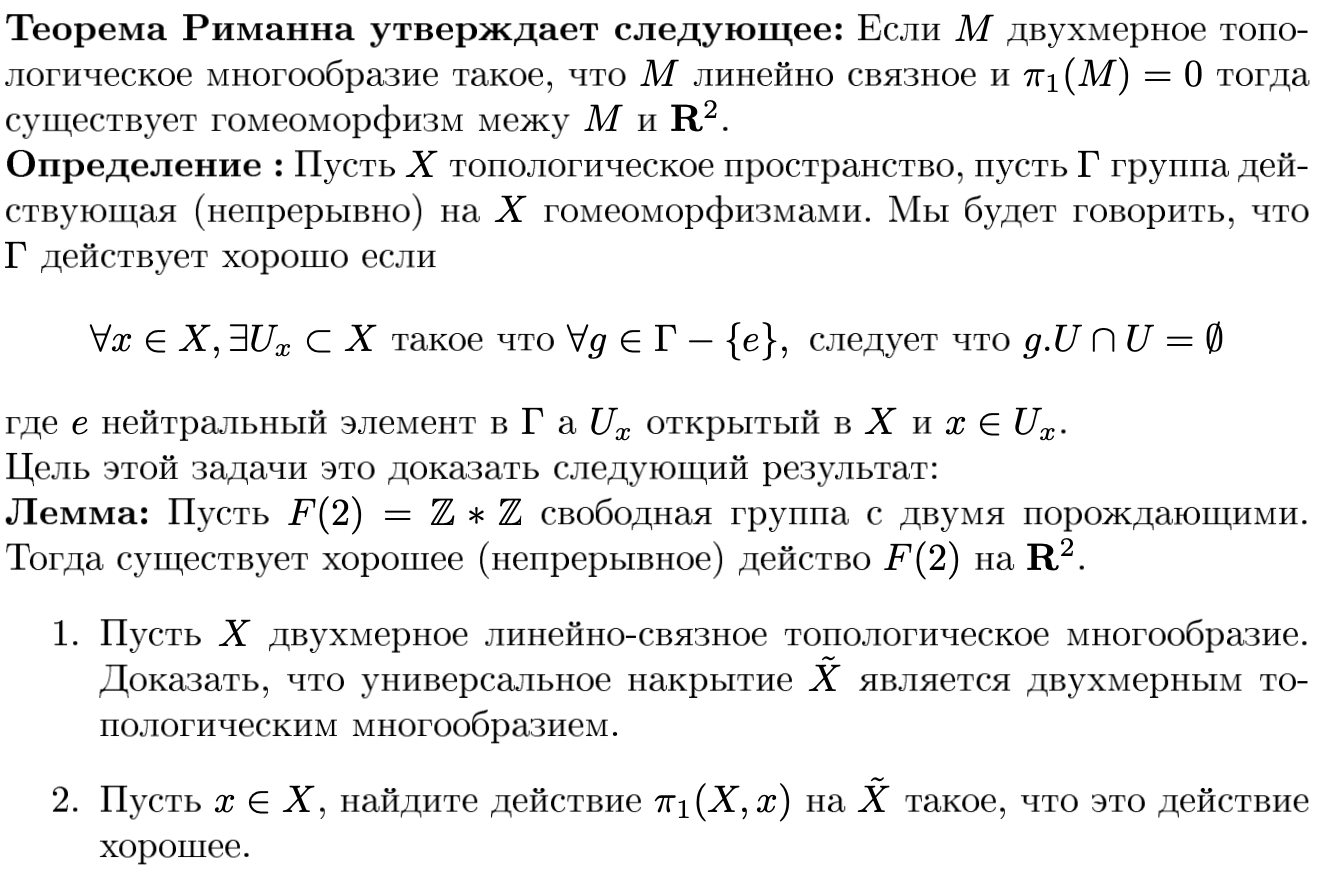
\includegraphics[width=1\textwidth]{photo_81.png}
\par
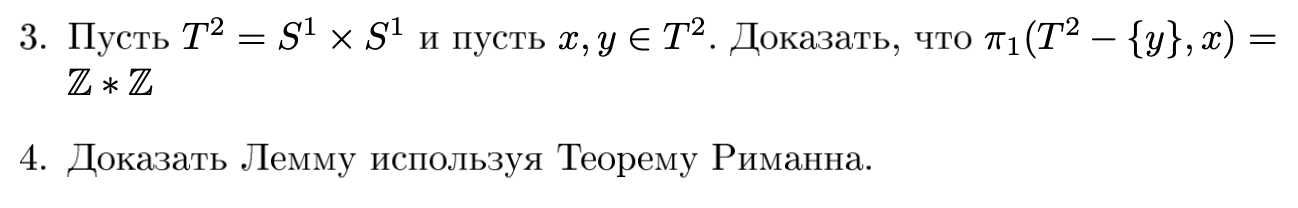
\includegraphics[width=1\textwidth]{photo_82.png}
\par Решение: :(
\par
\par
\end{large}
\end{document}
